% !TEX encoding = UTF-8 Unicode

\documentclass[twocolumn,10pt,a4j]{ltjsarticle}
\usepackage{kougai}

\title{VRデートアプリの提案}
\author{1932158 小池 周平  指導教員 須田 宇宙 准教授}
\date{ }

\begin{document}

\maketitle

\section{はじめに}


%背景

2015年9月に開催された「国連持続可能な開発サミット」でSDGsが掲げられた.この中に少子化も含まれており,その要因は,晩婚化の進展\cite{sasaki2012},交際率・婚姻率の減少\cite{naikakufu2019}などとされている.
晩婚化の進展が現状どの程度なのか調べたところ,平均初婚年齢は20年間で夫は2.6歳,妻は3.1歳増加している.
一方,18〜34歳の結婚意欲の調査結果によると,1987年〜2010年の結婚意欲はほとんど変化していない.
すなわち,「結婚はしたいけれど,良い相手に恵まれない」と思っている率が高く思われている\cite{naikakufu2019}.
これは,「出会いの場の減少」と「交際への不安」と言い換えることができる.
さらに,内閣府の調査によるとデートの経験がない男性は約4割いるとされている\cite{naikakufu2022}.
%問題点


以上のことから,出会ってからデートに進展するまでをサポートできれば,婚姻率上昇に繋げられるのではないかと考えた.
近年では,SNSやマッチングアプリを通じて利用者が増えている.
しかし,2人きりで会うことやデート未経験による不安を感じる人も少なくない\cite{prtimes,yoshimura2020}.
そこで,会う場を現実ではなく仮想空間で実施することで緊張や不安なく最初の接触を果たせるのではないかと考えた.


これらから,本研究では少子化改善を見据えて疑似的なデートの経験を積ませ,将来的な婚姻率上昇に繋がるVRデートアプリの開発を行うことを目的とする.



%目的
\section{VRデートアプリについて}
VR空間内でデートするアプリでは個別の問題点を以下のように改善するコンセプトを考案する.
まず,2人きりで会うことの不安については,VR空間内で擬似的にデートを行うことで改善できる.
次に,デートが未経験に対しては,デートの時間を40分〜1時間に設定し,アプリを自動進行することでアプリが主体となり未経験者の負担を軽減することができる.
デート時間の前半に共通の体験をしてもらい,後半はその体験についておしゃべりする時間としてお互いの性格を知る機会を設けることとした.


以上のことから私はVRデートアプリケーションを提案する.


\section{開発したアプリケーションについて}
開発したアプリケーションでできることについて説明していく.
このアプリケーションは主にPC,VRデバイスのブラウザを推奨としていて指定されたURLを入力する事で起動できる.
URLを入力した後,2端末から同タイミングでStartボタンを打ち込むことで接続が可能となる.
会話機能は本アプリには搭載されていないので外部の通話アプリを使用して会話をしてもらう.
アプリケーション内では端末がPCの場合視点を矢印キーの左右で替えることができる.
また,端末がVR機器であれば,画面内の2DボタンをVRボタンに切り替えると,VRとして画面が映し出すことができる.
本アプリケーションはデートを自動進行化しており,Startボタンを押した後は風景が流れていきそれを楽しむものとなっている.
自動進行の意図としては,デートの行動の制限し道筋を建てることでデート未経験者が失敗しないように配慮をしている.

\begin{figure}[h]
\begin{center}
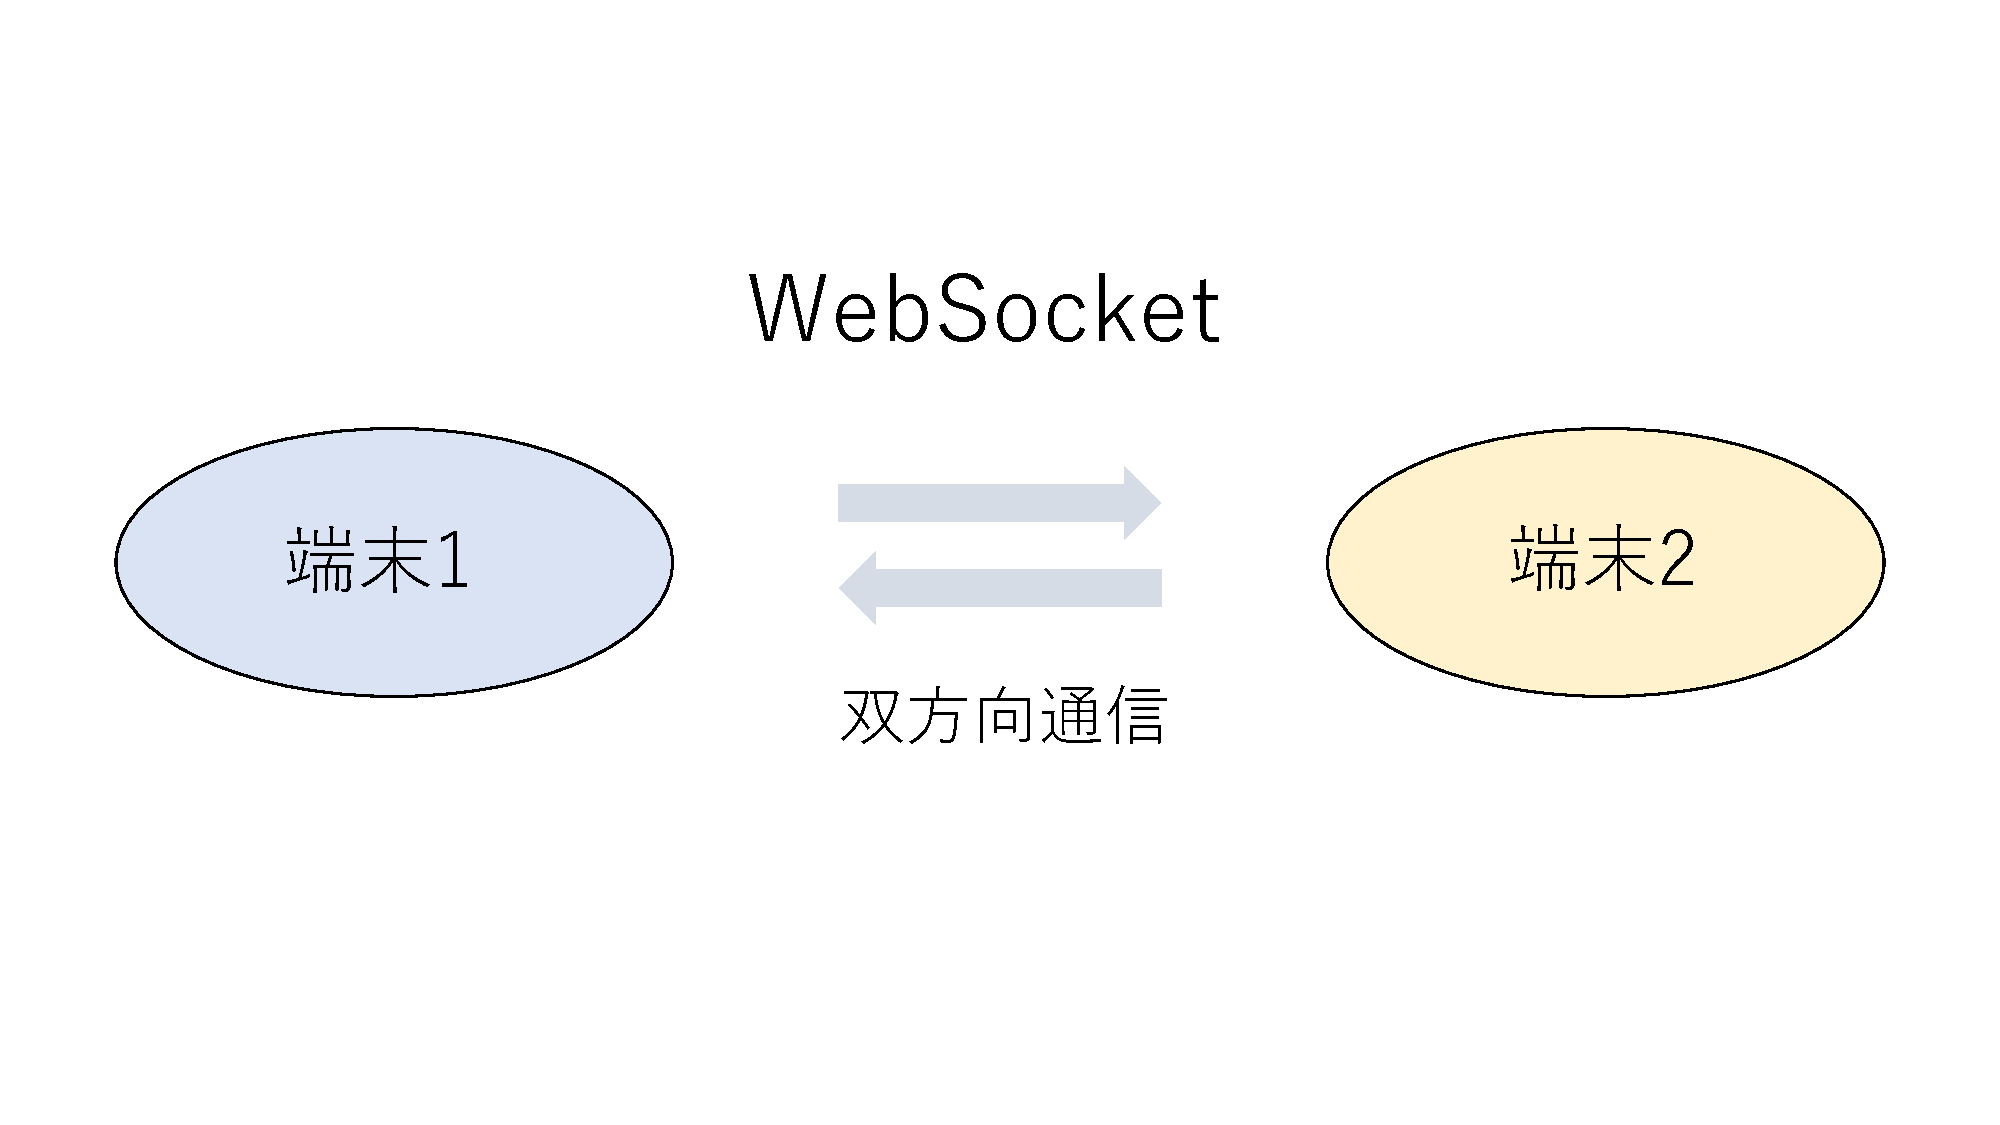
\includegraphics[width=75mm]{kougaisiryou.pdf}
\end{center}
 \caption{システム構成図}
\end{figure}

\section{おわりに}
本研究では少子化改善を見据えたデートアプリを開発した.このアプリを使用することで婚姻率・交際率の上昇を見込んでいる.

\begin{thebibliography}{99}
\bibitem{sasaki2012} 佐々木 尚之: ``不確実な時代の結婚-JGSSライフコース調査による潜在的稼得力の影響の検証'', 「家族社会学研究」,第24号,pp152-164(2012)
\bibitem{naikakufu2019} 内閣府: ``少子化対策の現状'', \url{https://www8.cao.go.jp/shoushi/shoushika/whitepaper/measures/w-2016/28webhonpen/html/b1_s1-1-3.html}, 2019/3/26参照
\bibitem{naikakufu2022}内閣府:``令和4年男女共同参画白書'',
\url{https://www.gender.go.jp/about_danjo/whitepaper/r04/gaiyou/pdf/r04_gaiyou.pdf},2022/6/14参照


\bibitem{prtimes}PRTIMES:``マッチングアプリは怖い?危ない目に合った?初めて会うまでの期間は!?徹底調査'',
\url{https://prtimes.jp/main/html/rd/p/000000016.000059676.html},2021/10/4参照
\bibitem{yoshimura2020} 古村 健太郎: ``成人のマッチングアプリ利用の背景-成人のマッチングアプリ利用に関する研究'', 「日本心理学会大会発表論文」,第84号,pc-006(2020)

\end{thebibliography}

\end{document}
